%!TEX root =  ../master.tex
%\section{Finite-range interactions in Two Dimensions}\label{sec:two-d}
\section{Two-dimensions}
In two dimensions, assuming a contact interaction, it is convenient to express eq.~\eqref{ere} as
\begin{equation}
\cot \left(\delta_{20}(p)\right)=\frac{2}{\pi}  \ln \left(p \tilde a_{20}\right)\ ,
\end{equation}
where
\begin{equation}
\tilde a_{20}=R_{20}e^{-\frac{2}{\pi}a_{20}}\ .
\end{equation}
Solving eq.~\eqref{IV pole} with $p=0$, $D=2$, and a finite cutoff $\Lambda$ gives
\begin{equation}\label{eq:C2}
C(\Lambda)=-\frac{2 \pi}{m \log \left(\tilde a_{20} \Lambda\right)}\ .
\end{equation}
Substituting this into eqs.~\eqref{FV pole} and ~\eqref{general luscher} gives the following relation,
\begin{equation}\label{eq:first 2d}
\frac{2}{\pi} \log \left(p\tilde a_{20}\right)=\lim_{\Lambda\to\infty}\left(-\frac{4}{m L^{2}} \sum_{\vec{q}}^{\Lambda} \frac{1}{E-\frac{\vec{q}^{2}}{m}}-\frac{2}{\pi} \log (\Lambda / p)\right)\ .
\end{equation}
The logarithmic dependence on $p$ makes eq.~\eqref{first 2d} difficult for analysis, particularly for small $p$.  Further, for $\tilde a_{20}$ sufficiently small (but positive)\footnote{ In 2-d the scattering length $\tilde a_{20}\ge 0$\cite{}.}, a bound state can occur, i.e. $p\to i\gamma$.  Then both sides of eq.~\eqref{first 2d} become complex which further complicates the analysis.   Also, the momentum-\emph{independent} logarithmic counterterm needed to regulate the infinite sum is not manifest in the above expression.  To make the counterterm manifest, and to address the issue of small $p$ states and bound states, we subtract $\frac{2}{\pi}\log\left(\frac{pL}{2\pi}\right)$ on both sides of the eq.~\eqref{first 2d}, giving
\begin{align}
\frac{2}{\pi} \log \left(\frac{2\pi \tilde a_{20}}{L}\right)&=\lim_{\Lambda\to\infty}\left(-\frac{4}{m L^{2}} \sum_{\vec{q}}^{\Lambda} \frac{1}{E-\frac{\vec{q}^{2}}{m}}-\frac{2}{\pi} \log \left(\frac{\Lambda L}{2\pi}\right)\right)\nonumber\\
%&=\lim_{\Lambda\to\infty}\left(\frac{1}{\pi^2} \sum_{\vec{q}}^{\Lambda} \frac{1}{\left(\frac{\vec{q}L}{2\pi}\right)^2-\frac{mL^2E}{4\pi^2}}-\frac{2}{\pi} \log \left(\frac{\Lambda L}{2\pi}\right)\right)\\
&=\lim_{\Lambda\to\infty}\left(\frac{1}{\pi^2} \sum_{\vec{q}}^{\Lambda} \frac{1}{\left(\frac{\vec{q}L}{2\pi}\right)^2-\left(\frac{pL}{2\pi}\right)^2}-\frac{2}{\pi} \log \left(\frac{\Lambda L}{2\pi}\right)\right)\ ,\label{eq:second 2d}
\end{align}
where in the last line we replaced $E\to p^2/m$.  Setting $N=\Lambda L/\pi$ and $\left(\frac{\vec{q}L}{2\pi}\right)^2=\vec{n}^2$ gives
\begin{align}
\frac{2}{\pi} \log \left(\frac{2\pi \tilde a_{20}}{L}\right)&=\frac{1}{\pi^2}\lim_{N\to\infty}\left( \sum_{|\vec{n}|\le \frac{N}{2}} \frac{1}{\vec{n}^2-\left(\frac{pL}{2\pi}\right)^2}-2\pi \log \left(\frac{N}{2}\right)\right)\nonumber\\
&=\frac{1}{\pi^2}S^\bigcirc_2\left(\left(\frac{pL}{2\pi}\right)^2\right)\ ,\label{eq:2d luscher}
\end{align}
where
\begin{equation}\label{eq:S2 spherical}
S^\bigcirc_2\left(x\right)\equiv\lim_{N\to\infty}\left( \sum_{|\vec{n}|\le \frac{N}{2}} \frac{1}{\vec{n}^2-x}-2\pi \log \left(\frac{N}{2}\right)\right)\ .
\end{equation}
Equation~\eqref{S2 spherical} is consistent with eq.~\eqref{spherical S} as long as we define\todo{Is this the right word?-T.L.} the limit
\begin{equation}
\lim_{D\to2}\counterterm_D^\spherical \left(\frac{N}{2}\right)^{D-2}=2\pi \log \left(\frac{N}{2}\right)\ .
\end{equation}
Equations~\eqref{2d luscher} and~\eqref{S2 spherical} represent our defintion of L\"uscher's formula in 2-D for a contact interaction. The expression encompasses both bound and scattering states.  Note the logarithmic dependence of the scattering length $\tilde a_{20}$ which requires an accompanying scale to render the argument of the logarithm dimensionless.  In our formulation, the accompanying scale is the length $L$ of the finite volume.   Finally, we note that for general finite-range interactions, the general L\"uscher formula in 2-D is
\begin{equation}\label{eq:full 2d luescher}
\cot(\delta_2(p))-\frac{2}{\pi}\log\left(\frac{pL}{2\pi}\right) = \frac{1}{\pi^2}S^\bigcirc_2\left(\left(\frac{pL}{2\pi}\right)^2\right)\ .
\end{equation}

\subsection{The scale invariant limit in 2 dimensions}
The logarithmic dependence of the scattering length and its accompanying scale is a consequence of the fact that in 2 dimensions, the interaction parameters of the Schr\"odinger equation are dimensionless.  \emph{Dimensionful} observables occur via dimensional transmutation \cite{} which requires some fiducial external scale, which in any finite-volume calculation is naturally given by the size of the volume.  An obvious question then arises about the unitary limit and how one approaches a scale-invariant limit in 2 dimensions, and whether or not such a limit exist.  We argue that such a limit does exist.

To see this, note that when $\tilde a_{20}=\frac{L}{2\pi}$ the LHS of eq.~\eqref{2d luscher} vanishes and we have an analogous quantization condition as in 3-D (when $a_{30}\to\infty$) and 1-D (when $a_{10}\to 0$).  In 3-D and 1-D, such a situation is akin to the unitary limit, once the infinite volume limit has been taken.  This limit can be done independently of taking $a_{30}\to\infty$ (3-D) or $a_{10}\to0$ (1-D).  However, in 2-D, because of the logarithmic dependence, the infinite volume limit $L\to\infty$ cannot be taken independently of $\tilde a_{20}$.  In particular, for the scale-invariant limit, one must take both $\tilde a_{20}\to \infty$ and $L\to\infty$ limits simultaneously \emph{such that} $L/\tilde a_{20}=2\pi$.  Such a procedure maintains the ``flatness" of the L\"uscher equation on the horizontal line at each step of the $\tilde a_{20}\to\infty$ and $L\to\infty$ extrapolation, and results in a non-trivial, scale-invariant, two-body system in 2-D.  \todo{You guys can probably say this better than me, I'm sure.  T.L.}

\subsection{Dispersion L\"uscher in 2 dimensions}
The discussion above is valid only in the continuum.  For a discretized lattice, an additional length scale is introduced that must be accounted for.  As is the case in both 3-D and 1-D, there exists a dispersion L\"uscher equation that is valid for the contact interaction and accounts for the discretization.  In \autoref{sec:counterterm/dispersion} we derive this dispersion L\"uscher formula for 2-D and only state the result here.  Identifying the lattice spacing $\epsilon=N/L$, we have
\begin{align}
\frac{2}{\pi} \log \left(\frac{2\pi \tilde a_{20}}{L}\right)&=\frac{1}{\pi^2}\left( \sum_{n_x,n_y=-\frac{N}{2}}^{\frac{N}{2}-1}\frac{1}{\vec{n}^2-\left(\frac{pL}{2\pi}\right)^2}-2\pi \log \left(\mathcal{L}_\square\frac{N}{2}\right)\right)\nonumber\\
&=\frac{1}{\pi^2}S^{\dispersion}_2\left(\left(\frac{pL}{2\pi}\right)^2\right)\ ,\label{eq:2d dispersion luscher}
\end{align}
where
\begin{equation}
\mathcal{L}_{\square}=\exp \left(\log (2)-G \frac{2}{\pi}\right)=1.116306393581637659468497 \ldots
\end{equation}
and $G$ is Catalan's constant.  

Given a contact interaction with coefficient appropriately tuned to the continuum scattering length $\tilde a_{20}$ and accounts for the discretization $\epsilon=N/L$ (see \autoref{sec:counterterm/dispersion}),
\begin{equation}
C(N/L)=-\frac{2 \pi}{m \log \left(\tilde a_{20} \mathcal{L}_\square \frac{N}{L}\pi\right)}\ ,
\end{equation}
the eigenvalues $x=\left(\frac{pL}{2\pi}\right)^2$ of Schr\"odinger's equation on a \emph{discretized} square lattice will exactly satisfy eq.~\eqref{2d dispersion luscher}.
\begin{figure}
\center
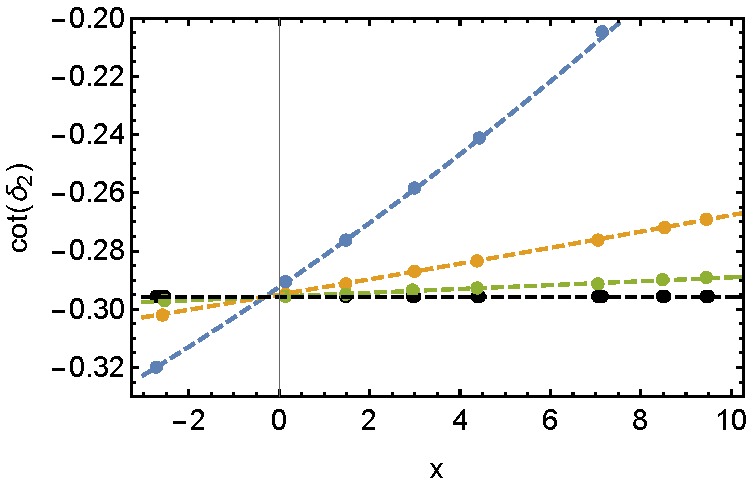
\includegraphics[width=.65\textwidth]{figure/luescher2d.pdf}
\caption{Results in 2-D using non-continuum eigenvalues $x=p^2L^2/4\pi^2$ of the Schr\"odinger equation with $N=10$, 20, and 40.  The interaction was tuned such that $\tilde a_{20}/L=.1$.  The colored points are obtained using $S^\bigcirc_2(x)$ with $N=10$ being furthest from a flat line and $N=40$ being closest.  The black points are obtained using $S^{\dispersion}_2(x)$  and exhibit the correct flat-line behavior.  The colored dashed lines are the derived induced momentum-dependent terms (see text) \todo{Need better figure. -T.L.}\label{fig:luescher2d}}
\end{figure}
This is depicted in \autoref{fig:luescher2d} by the black points which were calculated with $N=10$, 20, and 40.  Here the scattering length was set to $\tilde a_{20}/L = .1$, which allows for a bound state.  All black points lie on a flat line, indicating that our dispersion L\"uscher has correctly accounted for discretization effects.  On the other hand, if we use the same energies but insert them into continuum L\"uscher (eq.~\eqref{2d luscher}), as depicted by the colored points, momentum-dependent terms are induced and the flat line behavior is lost.

As was done in the 3-D\todo{still needs to be done.-T.L.} and 1-D cases, we can derive the functional form of the induced momentum-dependent terms.  The steps are identical to those done in the 3-D and 1-D cases, and so for conciseness we show only the end result.  Assuming an $x=\left(\frac{pL}{2\pi}\right)^2$ calculated on a \emph{discretized} lattice with lattice spacing $\epsilon=N/L$, we have
\begin{align*}
 \frac{1}{ \pi^{2}} S^\bigcirc_{2}\left(x\right)&=\frac{2}{\pi}\log\left(2\pi \frac{\tilde a_{20}}{L}\right)+ \frac{1}{ \pi^{2}} S^\bigcirc_{2}\left(x\right)- \frac{1}{ \pi^{2}} S^{\dispersion}_{2}\left(x\right)\\
 &=\frac{2}{\pi}\log\left(2\pi \frac{\tilde a_{20}}{L}\right)+\frac{1}{\pi^{2}} \left(\lim_{\eta\to\infty}\sum_{n\notin \operatorname{B.Z.}}^{|n|\le\frac{\eta}{2}} \frac{1}{n^{2}-x} -2\pi\log\left(\frac{\eta}{\mathcal{L}_\square N}\right)\right)\\
&=\frac{2}{\pi}\log\left(2\pi \frac{\tilde a_{20}}{L}\right)+\frac{1}{\pi^{2}} \left(\lim_{\eta\to\infty}\sum_{n\notin \operatorname{B.Z.}}^{|n|\le\frac{\eta}{2}}  \frac{1}{n^{2}} -2\pi\log\left(\frac{\eta}{\mathcal{L}_\square N}\right)\right) 
+\frac{1}{\pi^{2}}\sum_{n\notin \operatorname{B.Z.}} \frac{x}{n^{4}} +\frac{1}{\pi^{2}}\sum_{n\notin \operatorname{B.Z.}} \frac{x^2}{n^{6}}+\mathcal{O}(x^3)\\
&\equiv\frac{2}{\pi}\log\left(2\pi \frac{\tilde a_{20}}{L}\right)+\alpha_0(N)+\alpha_1(N) x+\alpha_2(N) x^2 +\mathcal{O}(x^3) \ .
\end{align*}
The coefficients $\alpha_i(N)$ have an implicit dependence on $N$ since the sums are restricted outside of the Brillouin zone.  Further, in 2-D the sums involved in $\alpha_i$ converge sufficiently fast and thus require no acceleration techniques.  We provide  
\begin{table}
\caption{The induced momentum-dependent terms to order $x^2$ due to a contact interaction using $S^\bigcirc_2(x)$ as a function of discretization $N$.  Here $x=\left(\frac{pL}{2\pi}\right)^2$ is a non-continuum eigenenergy.  \label{tab:induced terms in 2 d}}
\begin{tabular}{c|c}
$N$ & $\alpha_0(N)+\alpha_1(N) x+\alpha_2(N) x^2$\\
\hline
10 &$0.003446926 + 0.01065059589 x + 0.00018852319 x^2$\\
20 &$0.000862459 + 0.00261909878 x + 0.00001122531 x^2$ \\
40 &$0.000212552 + 0.00065179064 x + 6.92648\times10^{-7} x^2$ \\
\hline
\end{tabular}
\end{table}
the numerical values of $\alpha_i(N)$ in \autoref{tab:induced terms in 2 d} for the discretizations shown in \autoref{fig:luescher2d}.  They were also used to calculate the dashed colored lines in \autoref{fig:luescher2d}.


%Here we use a separable potential of the form
%\begin{equation}
%V(\bm p',\bm p)=\frac{4}{m}\mathcal{C}f(\bm p')f(\bm p)\ .
%\end{equation}
%One can show that the discrete box eigenvalues $x=\frac{mL^2E}{4\pi^2}$ satisfy the self-consistency equation
%\begin{equation}\label{eqn:SE}
%\frac{1}{\mathcal{C}}+\frac{1}{\pi^2}\sum_{\bm n\in\mathrm{B.Z.}}\frac{f\left(\frac{2\pi}{L}\bm n\right)^2}{\bm n^2-x}=0\ .
%\end{equation}
%where $\bm n\in\mathrm{B.Z.}$ represents $\bm n\in(-N/2,N/2]^2$ and $N$ is the number of sites per side of the box.  Note that $\mathcal{C}$ is dimensionless in 2-d.  With a little math and manipulation, the phase shift can be determined with this separable interaction,
%\begin{equation}\label{eqn:cot d}
%\cot \delta(p) = \frac{1}{f(p)^2}\left(-\frac{1}{\mathcal{C}}+\frac{2}{\pi}\int_0^\infty dq \ \mathcal{P}\frac{qf(q)^2}{p^2-q^2}\right)\ .
%\end{equation}
%
%\subsubsection{Specific potentials}
%Our first example uses the following separable potential,
%\begin{equation}\label{eqn:potential1}
%f(p)=\frac{1}{\sqrt{1+(p/\Lambda)^2}}\ .
%\end{equation}
%In this case one has
%\begin{equation}
%\frac{2}{\pi}\int_0^\infty dq \ \mathcal{P}\frac{qf(q)^2}{p^2-q^2}=\frac{2}{\pi}\int_0^\infty dq \ \mathcal{P}\frac{q}{(p^2-q^2)(1+(p/\Lambda)^2)}=\frac{2}{\pi}\frac{\log\left(\frac{p}{\Lambda}\right)}{1+(p/\Lambda)^2}\ .
%\end{equation}
%Equation~\eqref{eqn:cot d} becomes
%\begin{equation}\label{eqn:first phase shift}
%\cot\delta(p)=-\frac{1+(p/\Lambda)^2}{\mathcal{C}}+\frac{2}{\pi}\log\left(\frac{p}{\Lambda}\right)\ .
%\end{equation}
%Without loss of generality, we trade the dimensionless coefficient $\mathcal{C}$ with a dimensional (length) parameter $a_0$ via the relation
%\begin{equation}
%-\frac{1}{\mathcal{C}}=\frac{2}{\pi}\log(a_0\Lambda)\ .
%\end{equation} 
%Equation~\eqref{eqn:first phase shift} becomes
%\begin{equation}
%\cot\delta(p)=\frac{2}{\pi}\log(a_0p)+\frac{p^2}{2}\left[\frac{4\log(a_0\Lambda)}{\pi\Lambda^2}\right]\ .
%\end{equation}
%
%So we tested this potential and L\"uscher's formula is working.  Here we use the parameters
%\begin{align*}
%a_0&=2 \\
%L&=10 \\
%N&=100\\
%\Lambda&= 5\\
%\cot\delta(p)&=\frac{2}{\pi} \log (2 p)+0.0586348 \ p^2\ .
%\end{align*}
%With these parameters we determined the eigenenergies $x$ by numerically finding the roots of eq.~\eqref{eqn:SE} and then feeding these values through eq.~\eqref{eqn:S2}. The left panel of \autoref{fig:cotd1} shows these results.  The right panel uses $a_0=1$, which in this case supports negative $x$ solution.
%\begin{figure}
%\center
%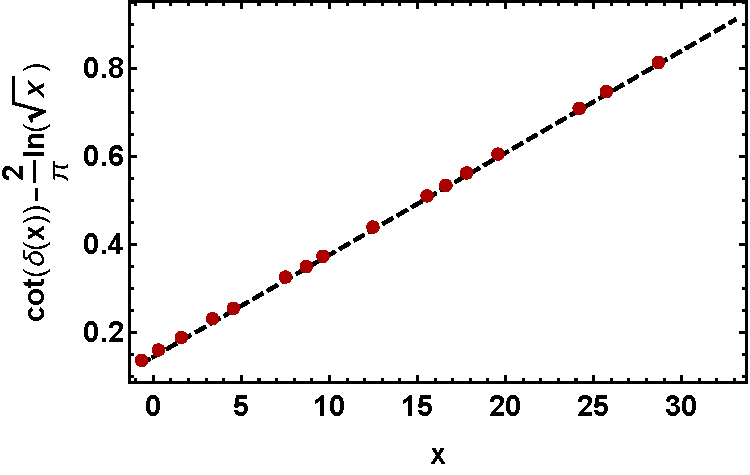
\includegraphics[width=.4925\textwidth]{figure/cotd1.pdf}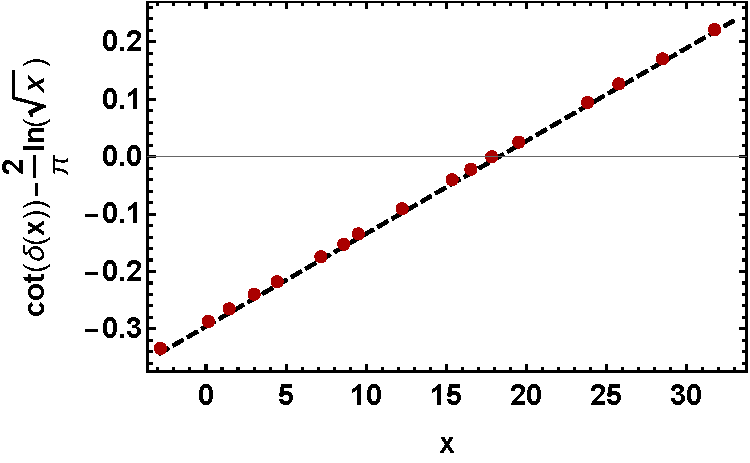
\includegraphics[width=.5075\textwidth]{figure/cotd4.pdf}
%\caption{Dashed line is the exact result, the red dots are numerical results.  The potential in this case is given by eq.~\eqref{eqn:potential1}.  Left panel does not support a negative energy solution ($2\pi a_0/L>1$), right panel does ($2\pi a_0/L<1$).\label{fig:cotd1}}
%\end{figure}
%The agreement between L\"uscher and exact is pretty good.  We have confirmed that as I increase $N$, the points converge to the exact line.  
%
%Our second example uses
%\begin{equation}\label{eqn:potential2}
%f(p)=\frac{1}{(1+(p/\Lambda)^2)^2}\ .
%\end{equation}
%Setting
%\begin{equation}
%\frac{-1}{\mathcal{C}}=\frac{2 \log (a \Lambda )}{\pi }-\frac{11}{6 \pi }\ ,
%\end{equation}
%we find 
%\begin{equation}
%\cot \delta(p)=\frac{2 \log (a p)}{\pi }+\frac{p^2 (24 \log (a \Lambda )-13)}{3 \pi  \Lambda ^2}+\frac{p^4 (24 \log (a \Lambda )-19)}{2 \pi  \Lambda
%   ^4}
%  +\frac{p^6 (8 \log (a \Lambda
%   )-7)}{\pi  \Lambda ^6} -\frac{p^8 (11-12 \log (a \Lambda ))}{6 \pi  \Lambda ^8}\ .
%\end{equation}
%Using the following parameters,
%\begin{align*}
%a_0&=2 \\
%L&=10 \\
%N&=100\\
%\Lambda&= 5\ ,
%\end{align*}
%We find good agreement between L\"uscher and the exact result, as shown in the left panel of~\autoref{fig:cotd23}.
%\begin{figure}
%\center
%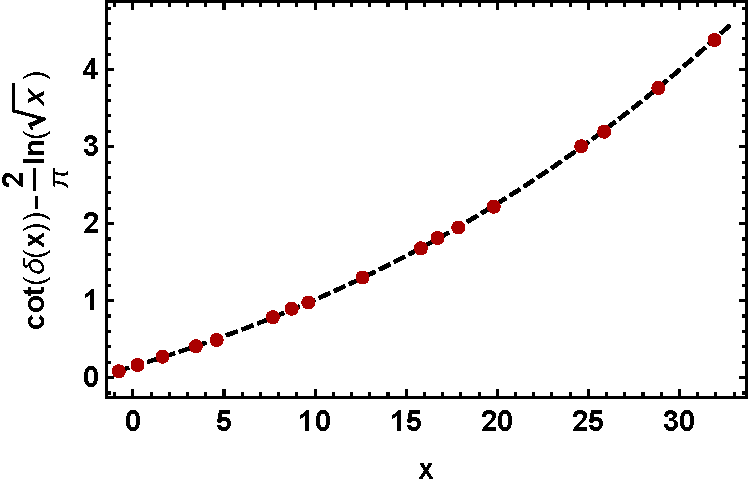
\includegraphics[width=.485\textwidth]{figure/cotd2.pdf}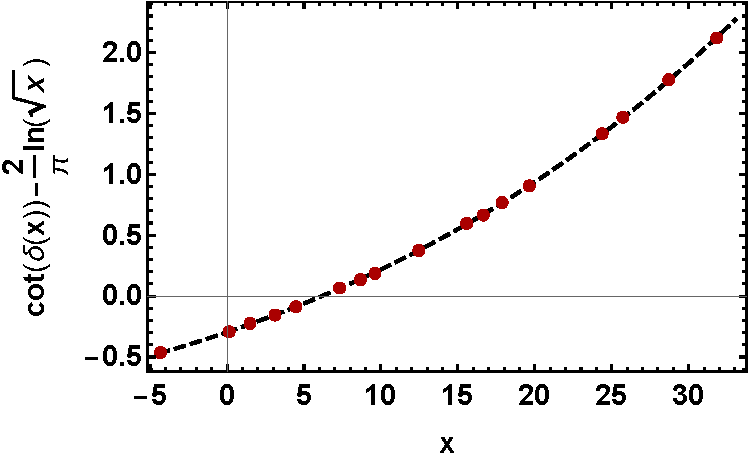
\includegraphics[width=.515\textwidth]{figure/cotd3.pdf}
%\caption{Dashed line is the exact result, the red dots are numerical results.  The potential in this case is given by eq.~\eqref{eqn:potential2}.  Left panel does not support a negative energy solution ($2\pi a_0/L>1$), right panel does ($2\pi a_0/L<1$).\label{fig:cotd23}}
%\end{figure}
%We also reduce the scattering length such that it supports a negative energy solution, $a_0=1$.  The right panel of~\autoref{fig:cotd23} shows this case.  Again, there is good agreement between exact and L\"uscher.